\documentclass[10pt]{article}

\usepackage[margin=1in]{geometry}
\usepackage{amsmath,amssymb}
\usepackage{booktabs}
\usepackage{graphicx}
\usepackage{float}
\usepackage{hyperref}
\usepackage[numbers,sort&compress]{natbib}

\title{SC-INR: Decoder-Side Sampling Consistency for Arbitrary-Scale Image Super-Resolution}
\author{Draft for internal review}
\date{May 2026}

\newcommand{\sinc}{\operatorname{sinc}}
\newcommand{\cell}{\mathbf{c}}
\newcommand{\coord}{\mathbf{x}}
\newcommand{\feat}{\mathbf{z}}
\newcommand{\freq}{\boldsymbol{\omega}}

\begin{document}
\maketitle

\begin{abstract}
Arbitrary-scale image super-resolution (ASISR) commonly represents an image as
a local implicit function queried at continuous output coordinates. Existing
Fourier implicit decoders such as LTE improve high-frequency reconstruction, but
their learned cell-conditioned phase allows the output footprint to directly
alter the local Fourier phase. This paper studies a more constrained
decoder-side formulation: the content function is predicted from image features,
while the output cell enters only through an analytic sampling response. We call
this family SC-INR. For a Fourier component observed through a box footprint,
the average response is a product of normalized sinc terms; SC-INR uses this
response to decouple feature-conditioned content from scale-conditioned
observation. Our current no-phase variant gives a stable small OOD PSNR gain
over LTE across three seeds, and substantially improves same-LR cross-scale
observation consistency in seed1 diagnostics. The feature-conditioned phase
final candidate shows positive OOD and All-scale mean gains over LIIF and LTE in
a three-seed benchmark; its comparison to the no-phase variant is reported as
seed1 context.
\end{abstract}

\section{Introduction}

ASISR aims to recover high-resolution images at arbitrary continuous scale
factors. Local implicit image functions, represented by coordinate-conditioned
MLPs over image features, provide a practical route to this setting
\citep{chen2021liif}. LTE improves this formulation by predicting local Fourier
coefficients and frequencies from image features, enabling stronger texture
modeling than a plain MLP \citep{lee2022lte}.

The current work revisits how the output cell enters such Fourier decoders. In
the ASISR query protocol, the cell is not an arbitrary scale token: it specifies
the output pixel footprint in the continuous image domain. In LTE, however, this
cell is fed to a learned phase map and directly shifts the Fourier argument.
This can improve fitting near training scales, but it also gives the network a
shortcut for moving local texture phase as a function of the requested output
footprint.

We therefore study \emph{decoder-side sampling consistency}. The central idea is
to separate the feature-conditioned continuous content from the scale-conditioned
observation. In SC-INR, the Fourier coefficient, frequency, and optional content
phase are functions of local image features only. The output cell affects the
decoded observation through an analytic sinc response derived from box averaging
a Fourier component. This is not a claim of whole-network scale equivariance:
the encoder, degradation model, and sampling protocol are not proven to commute
with scale transformations. The contribution is instead a constrained implicit
decoder contract that reduces arbitrary learned cell-conditioned phase
extrapolation.

\section{Method}

\subsection{Local Fourier Decoder}

Let \(E(I_{\mathrm{LR}})\) be the encoder feature map. For a query coordinate
\(\coord\), the decoder samples a local feature \(\feat\) and forms a relative
coordinate \(\delta\) to the local feature anchor. LTE predicts coefficients and
frequencies from \(\feat\), but also adds a learned phase term \(h_p(\cell)\):
\begin{equation}
  \cos\left(\pi(\freq(\feat)^\top \delta + h_p(\cell))\right).
\end{equation}
This creates a cell-specific local function \(f_{\feat,\cell}\), rather than a
single content function observed under different output footprints. Under scale
extrapolation, this branch is unconstrained: a larger footprint can alter where
the Fourier component appears, not merely how strongly it is observed.

\subsection{Analytic Observation Response}

Consider a one-dimensional Fourier component
\begin{equation}
  f(x)=A\cos(\pi \omega x+\phi).
\end{equation}
The box-averaged observation over a cell of width \(c\) is
\begin{equation}
  \frac{1}{c}\int_{x_0-c/2}^{x_0+c/2} A\cos(\pi \omega x+\phi)\,dx
  =
  A\cos(\pi \omega x_0+\phi)\sinc\left(\frac{\omega c}{2}\right),
\end{equation}
where \(\sinc(t)=\sin(\pi t)/(\pi t)\). For a two-dimensional rectangular
footprint, the separable response is
\begin{equation}
  W(\freq,\cell)=
  \sinc\left(\frac{\omega_h c_h}{2}\right)
  \sinc\left(\frac{\omega_w c_w}{2}\right).
\end{equation}
This is a signed sinc response. It can become negative for some
frequency-footprint pairs, which corresponds to the signed response of a box
filter rather than a guaranteed positive attenuation envelope.

\subsection{SC-INR Variants}

The final-candidate SC-INR predicts content terms from features:
\begin{equation}
  A=A(\feat), \qquad \freq=\freq(\feat), \qquad \phi=\phi(\feat),
\end{equation}
where \(A\) denotes the pre-MLP coefficient vector used by the decoder, not a
direct measurement of the final RGB image spectrum.
It uses signed bounded frequencies
\begin{equation}
  \freq(\feat)=\omega_{\max}\tanh(g_\omega(\feat)).
\end{equation}
The decoder input is
\begin{equation}
  A(\feat)\odot
  \left[
  \cos(\pi(\freq(\feat)^\top\delta+\phi(\feat))),
  \sin(\pi(\freq(\feat)^\top\delta+\phi(\feat)))
  \right]
  \odot W(\freq(\feat),\cell).
\end{equation}
Equivalently, the coefficient part can be viewed as a feature-level effective
amplitude
\begin{equation}
  A_{\mathrm{eff}}(\feat,\cell)=A(\feat)\odot W(\freq(\feat),\cell),
\end{equation}
which separates content-dependent coefficient strength from the
observation-dependent response of the output footprint. This interpretation
applies to the Fourier feature vector passed to the MLP decoder; because SC-INR
still uses an MLP, local ensemble, and residual upsampling, the full RGB
predictor should not be described as an exact analytic box integral.
The feature phase \(\phi(\feat)\) does not receive cell or scale. The previous
no-phase variant, denoted SC-INR-NoPhi, sets \(\phi=0\). We keep checkpoint and
raw-result compatibility names separate from paper display names; in older
result files, the raw key ``SC-INR'' refers to SC-INR-NoPhi, while the current
final-candidate SC-INR corresponds to raw key ``SC-INR+PhiZ'' in the seed1
historical file and to the cleaned raw key ``SC-INR'' in the seed2/seed3 files.

\section{Experiments}

\subsection{Protocol}

We use the inherited ASISR protocol with HR on-the-fly bicubic downsampling,
avoiding the unreliable local pre-generated LR benchmark files. Models are
trained on scales up to \(4\times\) and evaluated at in-distribution scales
\(\{2,3,4\}\) and OOD scales \(\{6,8,12,16,24,30\}\). PSNR is reported on
Set5, Set14, BSD100, and Urban100. Auxiliary diagnostics are currently computed
on BSD100 and Urban100 subsets for seed1. Paper benchmark tables are generated
from the canonical benchmark entry \texttt{artifacts/derived/benchmarks/}, which
records the raw key and canonical model name for every row.

\subsection{Seed1 Final-Candidate Benchmark}

\begin{table}[H]
\centering
\caption{Seed1 benchmark context. The final-candidate SC-INR was strongest in
seed1, but the current claim should use the three-seed summary in
Table~\ref{tab:final-multiseed}.}
\label{tab:seed1}
\begin{tabular}{lrrr}
\toprule
Model & ID PSNR & OOD PSNR & All PSNR \\
\midrule
LIIF & 30.9992 & 22.7111 & 25.4738 \\
LTE & 31.0450 & 22.6917 & 25.4761 \\
SC-INR-NoPhi & 31.0515 & 22.7471 & 25.5152 \\
SC-INR-NoPhi-Signed & 31.0567 & 22.7418 & 25.5134 \\
SC-INR & 31.1187 & 22.7766 & 25.5573 \\
LIIF-EQ & 31.1205 & 22.7469 & 25.5381 \\
\bottomrule
\end{tabular}
\end{table}

Table~\ref{tab:seed1} shows that the final-candidate SC-INR improves seed1 OOD
PSNR by \(+0.0849\) dB over LTE and by \(+0.0295\) dB over SC-INR-NoPhi. This
is the intended place to show the SC-INR vs SC-INR-NoPhi structural increment.

\subsection{Core Multi-Seed Result}

\begin{table}[H]
\centering
\caption{Core three-seed benchmark for LIIF, LTE, and SC-INR-NoPhi. The stable
multi-seed evidence currently belongs to the no-phase variant.}
\label{tab:multiseed}
\begin{tabular}{llrrr}
\toprule
Model & Split & Mean PSNR & Std. & Delta vs LTE \\
\midrule
LIIF & ID & 31.0301 & 0.0274 & -0.0485 \\
LIIF & OOD & 22.7251 & 0.0124 & +0.0177 \\
LTE & ID & 31.0786 & 0.0296 & +0.0000 \\
LTE & OOD & 22.7074 & 0.0137 & +0.0000 \\
SC-INR-NoPhi & ID & 31.0746 & 0.0203 & -0.0040 \\
SC-INR-NoPhi & OOD & 22.7581 & 0.0105 & +0.0507 \\
\bottomrule
\end{tabular}
\end{table}

Table~\ref{tab:multiseed} indicates that SC-INR-NoPhi gives a stable small OOD
PSNR gain over LTE, while its ID average is essentially tied with LTE. This is
consistent with the intended role of decoder-side sampling consistency: improving
scale extrapolation behavior rather than merely increasing training-scale
fitting.

\subsection{Final-Candidate Multi-Seed Result}

\begin{table}[H]
\centering
\caption{Final-candidate SC-INR three-seed benchmark. Deltas are paired seed
deltas against LIIF and LTE under the same benchmark protocol.}
\label{tab:final-multiseed}
\begin{tabular}{lrrrr}
\toprule
Split & Mean PSNR & Std. & Delta vs LIIF & Delta vs LTE \\
\midrule
ID & 31.0738 & 0.0582 & +0.0437 & -0.0048 \\
OOD & 22.7578 & 0.0316 & +0.0328 & +0.0504 \\
All & 25.5298 & 0.0403 & +0.0364 & +0.0320 \\
\bottomrule
\end{tabular}
\end{table}

Table~\ref{tab:final-multiseed} shows that the final-candidate SC-INR retains
the OOD and All-scale PSNR advantage over LTE and is positive over LIIF across
ID, OOD, and All splits. We keep SC-INR vs SC-INR-NoPhi as seed1 context rather
than foregrounding seed2/seed3 differences between those two internal variants.

\subsection{Cross-Scale Observation Consistency}

\begin{table}[H]
\centering
\caption{Seed1 same-LR cross-scale observation consistency. Larger consistency
PSNR indicates closer agreement when outputs at larger scales are compared to
the \(4\times\) observation under the same LR input.}
\label{tab:consistency}
\begin{tabular}{llrr}
\toprule
Model & Dataset & Consistency PSNR & Delta vs LTE \\
\midrule
LTE & BSD100 & 44.1914 & +0.0000 \\
SC-INR-NoPhi & BSD100 & 52.8053 & +8.6140 \\
LTE & Urban100 & 39.2983 & +0.0000 \\
SC-INR-NoPhi & Urban100 & 47.0694 & +7.7712 \\
\bottomrule
\end{tabular}
\end{table}

The large consistency gains in Table~\ref{tab:consistency} support the mechanism
that removing learned cell-conditioned phase is consistent with improved
same-LR cross-scale agreement. However, diagnostic LTE variants with weakened
cell response and SC-INR-NoSinc can also score highly on consistency; these
numbers must be interpreted jointly with reconstruction quality and
footprint-oracle diagnostics.

\subsection{Footprint Oracle Diagnostic}

Same-LR consistency alone cannot distinguish a footprint-aware decoder from a
cell-insensitive decoder. We therefore add a small seed1 diagnostic that keeps
the \(4\times\) LR input and query grid fixed, changes only the decoder cell,
and compares the output to a discrete HR box-average oracle at the same query
locations. The oracle is a piecewise-constant proxy from the available HR image,
so it is a diagnostic target rather than a true continuous-scene integral.

\begin{table}[H]
\centering
\caption{Seed1 footprint-oracle diagnostic on BSD100 and Urban100 first 10
images. Cell multiplier \(m\) is relative to the native \(4\times\) query grid.
Lower RMSE is better.}
\label{tab:footprint-oracle}
\begin{tabular}{lrrrr}
\toprule
Model & Oracle RMSE \(m=2\) & Oracle RMSE \(m=4\) &
Tracking RMSE \(m=2\) & Tracking RMSE \(m=4\) \\
\midrule
LTE & 0.02504 & 0.02309 & 0.03077 & 0.04834 \\
LTE-NoCellPhase & 0.02611 & 0.02653 & 0.03237 & 0.05134 \\
SC-INR-NoPhi & 0.02476 & 0.02057 & 0.03069 & 0.04708 \\
SC-INR & 0.02464 & 0.02148 & 0.03062 & 0.04745 \\
SC-INR-NoSinc & 0.02612 & 0.02750 & 0.03237 & 0.05134 \\
\bottomrule
\end{tabular}
\end{table}

Table~\ref{tab:footprint-oracle} shows that SC-INR tracks the footprint oracle
better than the cell-insensitive NoSinc control under this small diagnostic,
while LTE-NoCellPhase and SC-INR-NoSinc have zero cell sensitivity and therefore
inherit the oracle-change error. SC-INR-NoPhi is slightly stronger than the
final feature-phase SC-INR on this diagnostic, so this result should be read as
support for the analytic footprint-response mechanism, not as a claim that the
final variant is best on every auxiliary metric.

\subsection{LTE-to-SC-INR Mechanism Gate}

The footprint-oracle diagnostic compares output behavior, but the central
mechanism claim is more specific: LTE lets the cell directly change a learned
phase signal, whereas SC-INR lets cell change a pre-MLP analytic response. We
therefore add a crop-based seed1 gate that uses the same images, query points,
and cell multipliers to record LTE's isolated \(h_p(c)\), SC-INR's active
response, and the footprint-oracle errors. This diagnostic uses BSD100 and
Urban100 first 5 images, center \(64\times64\) HR crops, and 256 query points
per image; it is intentionally a mechanism gate, not a replacement for the
full-image footprint oracle or the multi-seed benchmark.

\begin{table}[H]
\centering
\caption{Unified LTE-to-SC-INR mechanism diagnostic, averaged over cell
multipliers \(m=2,4\). Lower RMSE is better. Signal deltas are measured against
the native \(m=1\) cell.}
\label{tab:lte-scinr-mechanism}
\begin{tabular}{lrrrr}
\toprule
Model & Oracle RMSE & Tracking RMSE & \(h_p(c)\) delta & Active response delta \\
\midrule
LTE & 0.02623 & 0.04198 & 0.51528 & -- \\
LTE-NoCellPhase & 0.02714 & 0.04353 & -- & -- \\
LTE-PhaseZ & 0.02695 & 0.04353 & -- & -- \\
SC-INR & 0.02512 & 0.04113 & -- & 0.30812 \\
SC-INR-NoPhi & 0.02476 & 0.04101 & -- & 0.29938 \\
SC-INR-NoSinc & 0.02729 & 0.04353 & -- & 0.00000 \\
\bottomrule
\end{tabular}
\end{table}

Table~\ref{tab:lte-scinr-mechanism} directly supports the intended mechanism
distinction. LTE has a non-zero learned cell-phase signal; NoCellPhase and
NoSinc remove the active cell response and therefore inherit the oracle-change
error; SC-INR keeps a non-zero analytic response and tracks the crop oracle
slightly better than LTE and NoSinc. The table should still be interpreted
narrowly: the phase norm and response norm are not the same physical quantity,
and this crop-based diagnostic does not prove that sinc is the unique cause of
the benchmark gain.

\subsection{Selected Qualitative Examples}

\begin{figure}[H]
\centering
\begin{minipage}{0.48\linewidth}
\centering
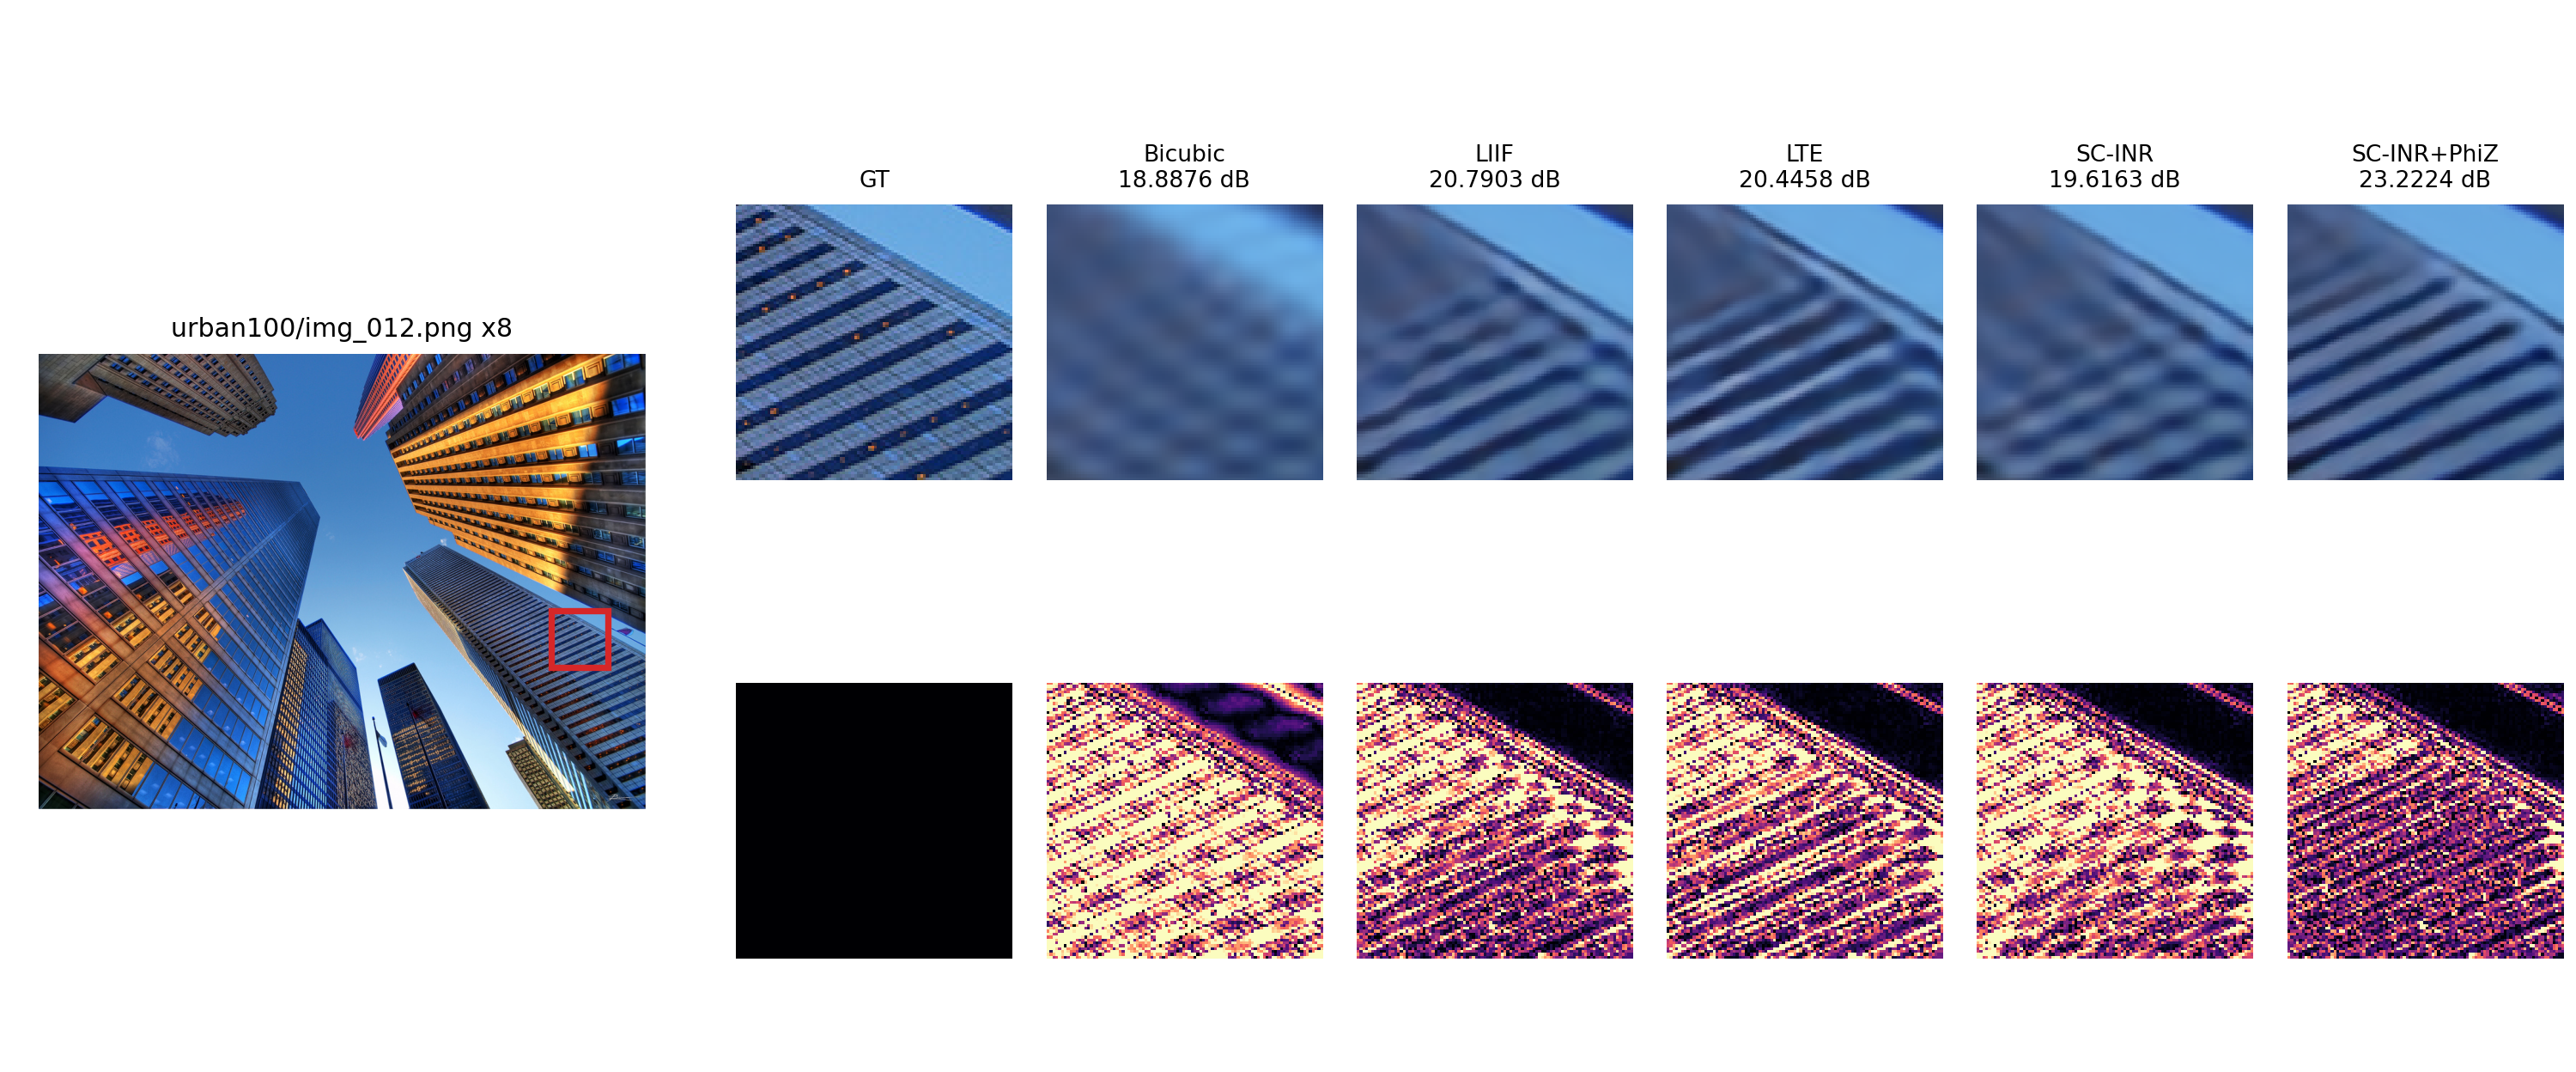
\includegraphics[width=\linewidth]{figures/urban100_img012_x8.png}
\end{minipage}
\hfill
\begin{minipage}{0.48\linewidth}
\centering
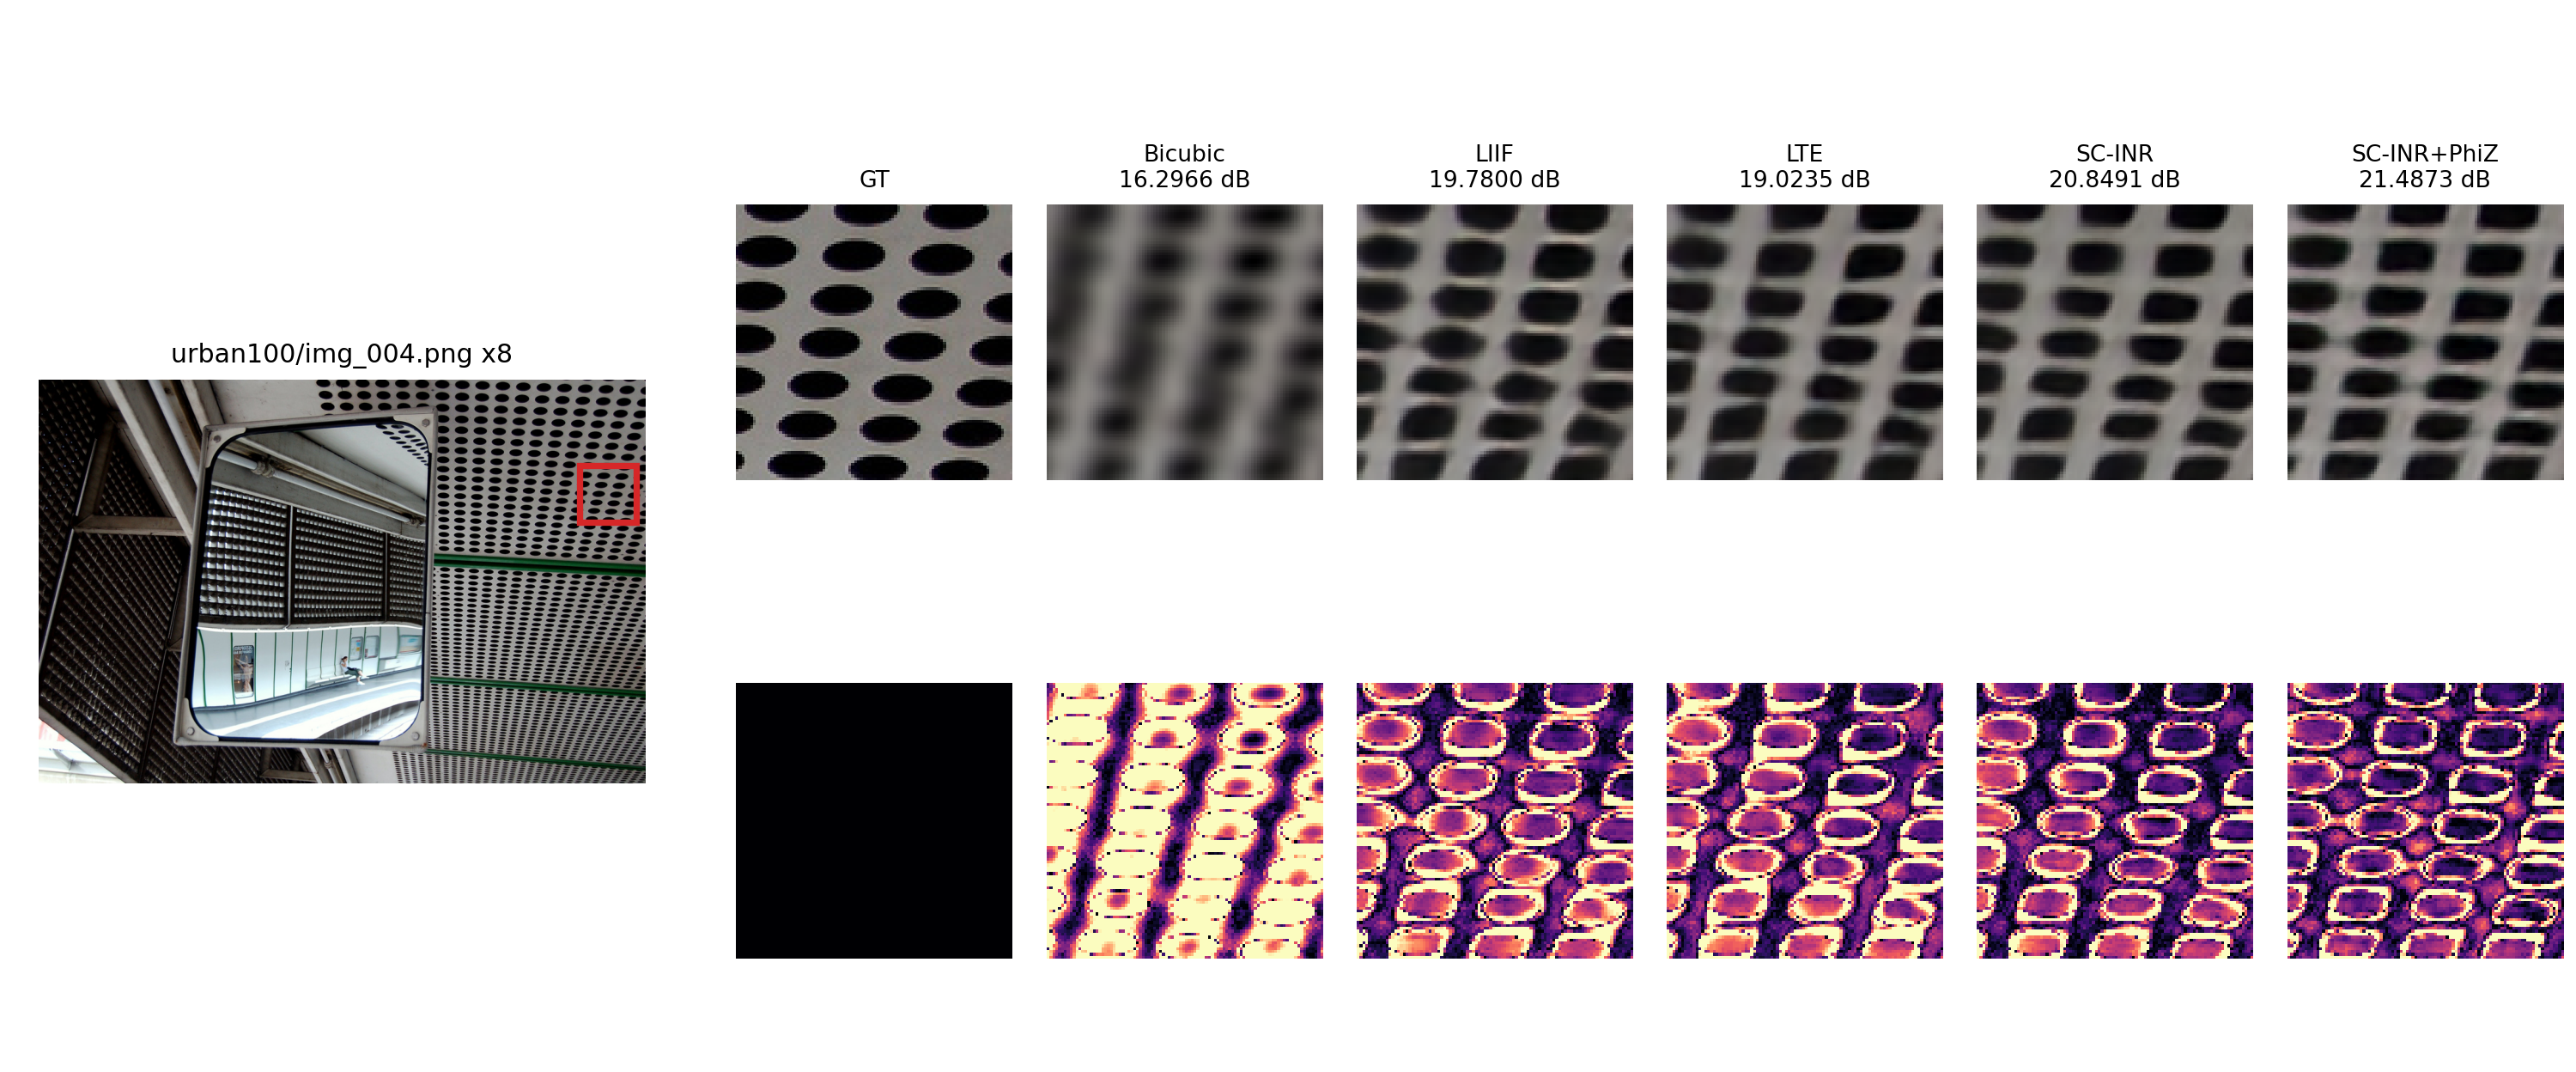
\includegraphics[width=\linewidth]{figures/urban100_img004_x8.png}
\end{minipage}
\caption{User-confirmed selected Urban100 \(8\times\) examples where the
final-candidate SC-INR shows clearer local structure than LTE. These are
selected examples, not evidence of average visual quality.}
\label{fig:qualitative}
\end{figure}

\section{Limitations and Next Steps}

The current evidence is not yet a complete paper claim. First, final-candidate
SC-INR now has three-seed benchmark evidence against LIIF and LTE, but auxiliary
metrics for the final candidate remain seed1-only. Second, the w/o-sinc ablation
is still single-seed and should not be used as a
unique causal proof of the analytic response. Third, same-LR consistency can
reward cell-insensitive behavior; the footprint-oracle diagnostic partly closes
this gap but remains a seed1 small-sample HR proxy, not a proof that the final
RGB output is an exact box-footprint observation. Finally, PSNR does not fully
measure perceptual texture quality; qualitative crops and texture-sensitive
metrics must remain part of the evidence package.

\section{Conclusion}

SC-INR reframes output scale in Fourier implicit ASISR decoders as an
observation footprint rather than a learned phase shortcut. The current results
support decoder-side sampling consistency as a useful principle: SC-INR-NoPhi
shows stable small OOD gains and substantially better cross-scale observation
consistency, while the final-candidate feature-phase SC-INR preserves the OOD
and All-scale PSNR gain over LTE and improves over LIIF on average.
The next critical step is to close the remaining evidence gap with final-candidate
auxiliary metrics, broader footprint-correctness checks, and carefully audited
qualitative evidence.

\bibliographystyle{plainnat}
\bibliography{references}

\end{document}
